\documentclass[12pt]{article}
\renewcommand{\baselinestretch}{1.5}
\usepackage{graphicx}
\usepackage{subfigure}
\usepackage{amsmath}
\usepackage{amsfonts}
\usepackage{euscript}
\usepackage{amssymb}
\usepackage{fancyhdr}
\usepackage[all]{xy}
\textheight 9in
\textwidth 6.5in
\voffset -1in
\hoffset -.75in
               
%\pagestyle{fancy}
\pagenumbering{gobble}
%\rhead{Austen Kelly\\Onyen: akellyca}
%\lhead{Comp 550 Homework \#1}

\begin{document}
\centerline{\large \textbf{COMP 580 Project Proposal}}
\centerline{Anthony Kan, Austen Kelly, Kent Torell}
\vskip 0.5cm

\textbf{\large Key Idea}\\
\textbf{Basic Layout:}\\
\indent This project, which has the working title Blind Maze is designed to be a fairly difficult two player cooperative game which requires a high level of participation and communication from both players.  One of the players will be called the Maze Runner (or Runner for short) and will be in charge of moving the virtual game piece through the maze.  The Runner has no knowledge of the layout of the maze, the starting position, or where the finishing spot will be. The Runner has access to four buttons: walk forward, turn 90$^\circ$ counterclockwise, turn 90$^\circ$ clockwise, and a button to check if they are in the correct ending spot.  If the checking button is pressed and the game piece is not in the correct spot the Runner will hear an error sound and lose a life, if all three lives are used the game ends with a failure game over.\\
\indent The other player will be called the Director. Their job is to direct the Runner through the maze without having any firm knowledge as to where the Runner currently is. The Director has access to a 3D printed board which has a maze overlaid on top of it (more details in the Architecture section).  There will also be non-maze related objects that correspond to sounds that the Runner will be able to hear and use to describe to the Director so that the two may be able to pinpoint where in the map the Runner's game piece is.\\
\textbf{Gameplay:}\\
\indent Each game starts with the Runner's game piece being randomly spawned somewhere on our 10x10 tile maze.  The runner will describe the sounds they hear to the Director, who will use the map to infer the location of the Runner.  The louder the sound is the closer the game piece is to that sound.  Once the starting location is discovered the Directors goal is to direct the Runner through the maze to a randomly selected finishing location that is at least 15 steps away from the starting location (generated by the computer, not the Director).  Once both the Director and the Runner believe they are in the correct spot the Runner presses the check button.  If the game piece is in the correct location the players will have successfully completed the game.  If the piece is in the wrong location then the error sound will play, the players will lose a life, they must continue trying to find the correct spot.\\

\textbf{\large Target Users}\\
\indent The target users for this game will be Maze Day visitors.  While the primary focus of the game is to create a game which we believe will be easier for blind individuals, we do not believe that this is the only use.  Anyone who is able to hear and wishes to build their communication and description skills could benefit from playing this game, as the game forces two individuals to communication constantly in order to achieve a shared goal.  We can also have the added benefit of offering sighted individuals a blind perspective by offering them a blindfold if they are to be the Director; or by simply having them play as the Runner where sight cannot be used at all.\\

\textbf{\large Architecture Diagram}\\
%Create a diagram describes high-level components of your system, and how they interact. For each module in the diagram, explain its primary function(s) and what technology/hardware it will use. If your project is a game, please include a related story board or flow diagram.
\indent \textbf{Runner:} The Runner will not be actually moving through the game-world, but instead virtually moving using a four button game pad. The four buttons will function as follows: one square forwards, turn left in place, turn right in place, and the check button. After the runner chooses their move, the audio portion will adapt accordingly, as the input gets sent to the virtual map.\\
\indent \textbf{Maze:} The following is an example of a maze that will be 3D printed as our physical non-reactive game board, with a virtual maze programmed into the computer, where the location of the runner will be virtually kept track of:
\newpage
\begin{figure}[ht]
\subfigure{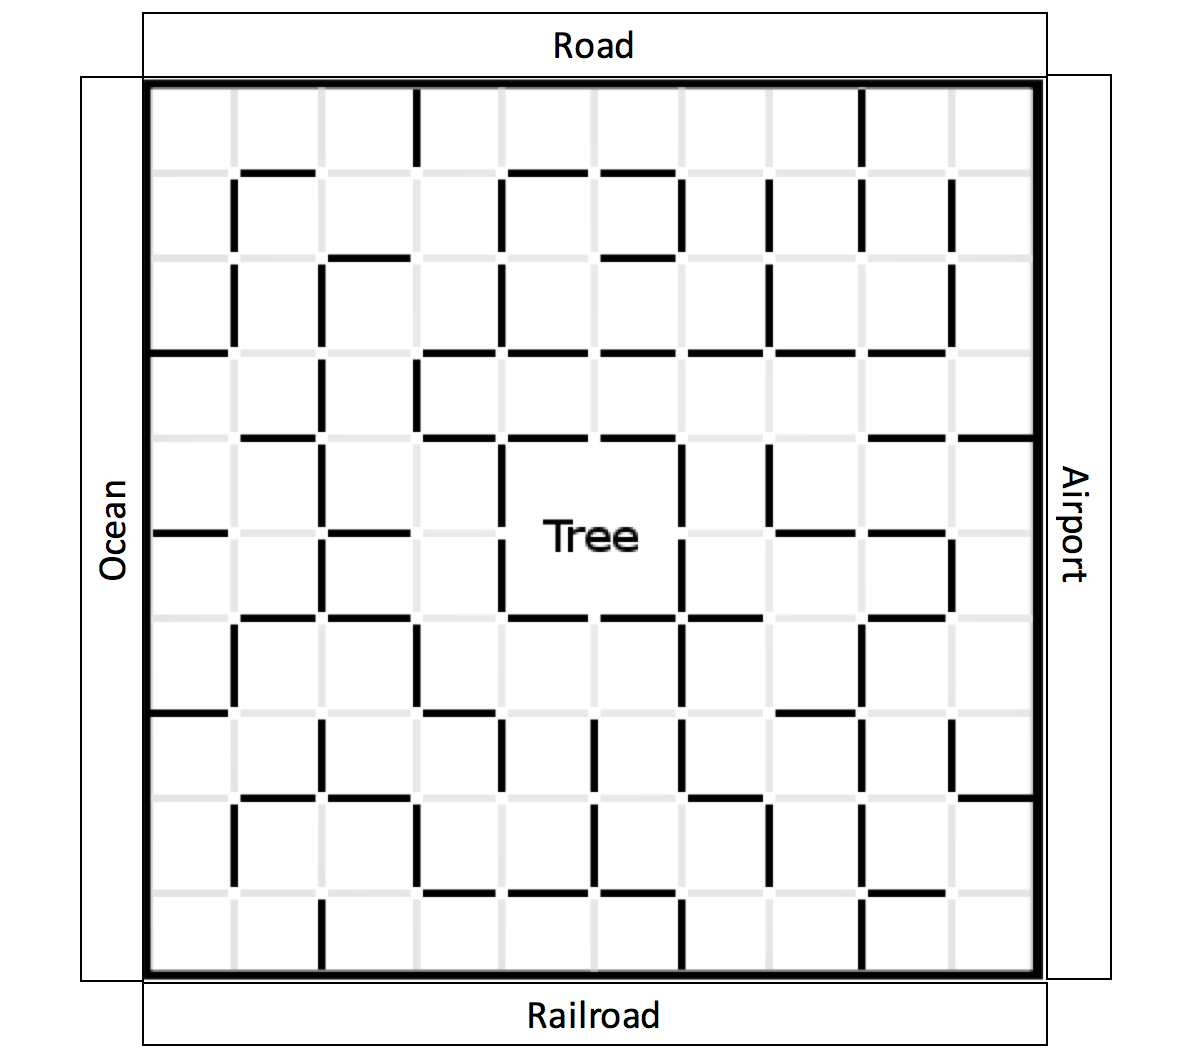
\includegraphics[width=0.9\textwidth]{maze_img.jpeg}}
\end{figure}

\indent This maze is just an example of what the final product might look like; we have not finalized what sounds we want, or where we are going to put them.  The black lines indicate raised walls that would act as the walls of the maze which the game piece cannot pass through.  The grey lines will be indented into the 3D print so that the Director can tell where one cell ends and another cell begins without actually seeing the board.  In this example the Runner might hear waves and seagulls coming from the ocean while the Director might feel ripples on the water and maybe a dock or a boat.  The railroad might sound like a train running across a set of tracks or maybe a railroad crossing bell, and might feel/look like a set of tracks with a train on it.  As for the airport we thought we would print a run way with an airplane on it which might give off the sound of airplanes flying through the air.  The road would probably be printed with a car on it and would sound like cars driving by and maybe the occasional honk.  The tree in the middle will have sounds of birds coming out of it or maybe branches rustling in the wind.\\
\indent The sounds played to the runner will be a function of the runner's location in the maze. The sound will be directed in the left/right headphone for orientation. If the runner walks towards something, that sound will increase and steps sounds will play to indicate that they have successfully moved. If the runner accidentally walks into a wall, a thud sound will play.\\

\textbf{\large Technologies and Hardware}\\
%Describe each library/framework and hardware system you plan to use for this project. (What is its main purpose, and why have you chosen it to use for this project?) In this section, also include how you plan to make your code available to target users. (Hosted on website, available through app store, etc.)

\indent For this game we need two computers, one that only needs a voice communicator (Skype Ventrillo, Teamspeak, etc.), and one that needs to be able to run Python 2.7 along with having a voice communicator running simultaneously.  In addition we need two pairs of stereo headphones and two microphones so that the two participants can communicate with one another.  The headphones must be stereo so that the Runner can properly locate where the sounds are coming from.  In addition we will need a space large enough to hold our maze, which will be printed in a 20''x20'' area of 25 2''x2'' blocks laid out in a square, each block containing a 2x2 piece of the overall maze, with extra room on the sides for the side sounds.  We will also build a controller for the Runner to use out of 4 buttons, these can be made using any kind of button, as long as the button is big and has a tactile click when it activates.  As for the 3D printing, we plan on using stereo lithography printer as we have access to that type of printer and believe it is the best quality for what we want.\\
\indent Our plan is to use Python 2.7 to run the majority of the game.  The only library that we currently anticipate using is the pygame library as they have a built in sound library that we intend to use.  Since we don't require a fancy GUI (only really necessary for debugging purposes) we don't expect to use anything too crazy for visuals.\\
\indent We are not sure exactly how we plan on sharing this game in the future as it requires a few pieces of hardware that might not be easy to mass distribute.  As for the code we are putting everything on GitHub and running it with python, making the code itself easily accessible to all.\\

\textbf{\large Team Logistics}\\
\textbf{Team members:} Kent Torell (torell), Austen Kelly (akellyca), Anthony Kan (akan)\\
\textbf{Point person:} Kent Torell\\
\textbf{Maintenence:} We will maintain our code on Github. \\
\textbf{Division of Labor:} The breakdown of coding responsibility is tentatively as follows:\\
\indent Kent: 3D printing, controller input and functionality.\\
\indent Austen: Maze design, volume control/playback output.\\
\indent Anthony: Sound clip generation, 3D model design. 



\end{document}









